\section{Convex functions}
\subsection{Extended-valued functions}
\begin{definition}[Extended-valued function]
    A function $f: \R^n \longrightarrow \R$ is \emph{extended-valued} if its domain is $\R^n$ and its range is $\bar{\R} := \R \cup \{+\infty\}$.
\end{definition}

\begin{example}[Indicator function]
    We consider the indicator function of interval $[a, b]$:
    \begin{equation*}
        \ind_{[a,b]}(x) := \begin{cases*}
            0 & if $x\in[a,b]$ \\
            +\infty & otherwise
        \end{cases*}
    \end{equation*}
    \begin{figure}[H]
        \centering
        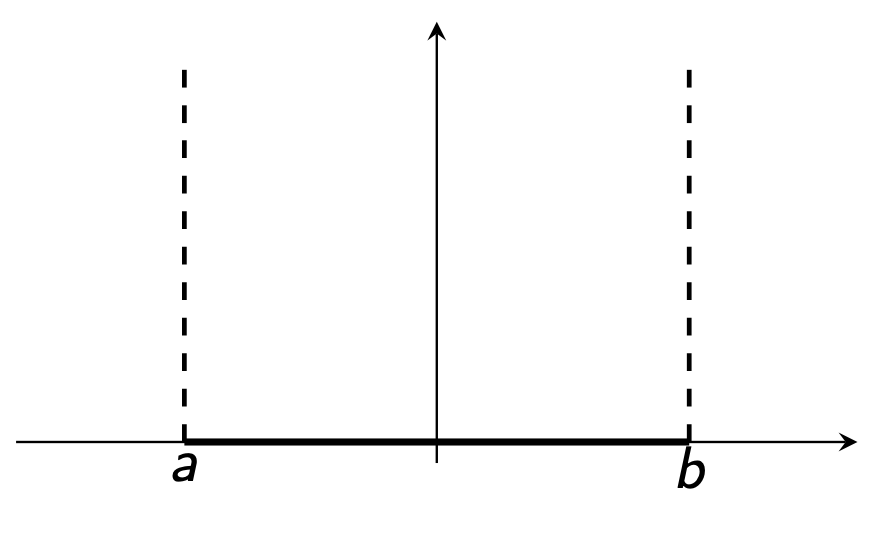
\includegraphics[width=.4\textwidth]{convex-functions/indicator.png}
    \end{figure}
\end{example}

\begin{definition}[Effective domain]
    The \emph{effective domain} of $f:\R^n\longrightarrow\bar{\R}$ is the set of points where $f$ is finite:
    \begin{equation*}
        \dom f := \set{x\in\R^n}{f(x)<+\infty}
    \end{equation*}
\end{definition}

A function is said to be \emph{proper} if its effective domain is non-empty: $\dom f \neq \emptyset$.

\subsection{Definition and first properties}
\begin{definition}[Convex function]
    A function $f:\R^n\longrightarrow\bar{\R}$ is \emph{convex} if its graph is below any line connecting two points of the graph $(x, f(x))$ and $(y, f(y))$. That is:
    \begin{equation*}
        \forall x,y\in\R^n, \forall\theta\in[0,1], \quad f(\theta\cdot x + (1-\theta)\cdot y) \leq \theta\cdot f(x) + (1-\theta)\cdot f(y)
    \end{equation*}
\end{definition}

\begin{definition}[Concave function]
    A function $f:\R^n\longrightarrow\bar{\R}$ is \emph{concave} if $-f$ is convex. That is:
    \begin{equation*}
        \forall x,y\in\R^n, \forall\theta\in[0,1], \quad f(\theta\cdot x + (1-\theta)\cdot y) \geq \theta\cdot f(x) + (1-\theta)\cdot f(y)
    \end{equation*}
\end{definition}

\begin{definition}[Epigraph]
    The \emph{epigraph} of a function $f:\R^n\longrightarrow\bar{\R}$ is the set of points lying above the graph of $f$:
    \begin{equation*}
        \epi f := \set{(x, t)\in\R^n\times\R}{f(x)\leq t}
    \end{equation*}
\end{definition}

\begin{property}[Convexity and epigraph]
    A function $f:\R^n\longrightarrow\bar{\R}$ is convex if and only if its epigraph is a convex set.

    \begin{figure}[H]
        \centering
        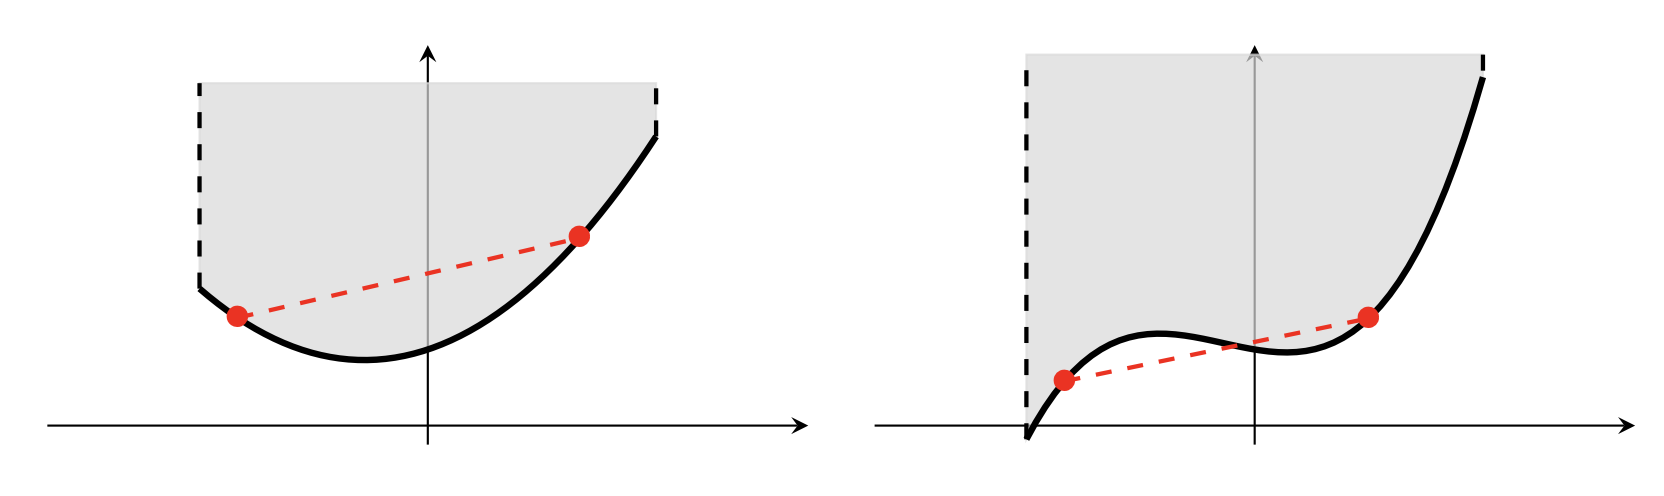
\includegraphics[width=.7\textwidth]{convex-functions/epigraph.png}
    \end{figure}
\end{property}

The following property allows to check the convexity of a multivariate function $f$ by checking the convexity of functions of one variable.
\begin{property}
    Let $f:\R^n\longrightarrow\bar{\R}$ be a function, and let $x\in\dom f$. We define:
    \begin{equation*}
        \begin{aligned}
            g_{x,v} : \R &\longrightarrow \bar{\R} \\
            t &\longmapsto f(x+tv)
        \end{aligned}
    \end{equation*}
    with $\dom g_{x,v} = \set{t\in\R}{x+tv\in\dom f}$. Then, $f$ is convex if and only if $g_{x,v}$ is convex in $t$ for all $x\in\dom f$ and all $v\in\R^n$.
\end{property}

\begin{definition}[Sublevel sets]
    Let $f:\R^n\longrightarrow\bar{\R}$ be a function. The \emph{sublevel set} of $f$ at level $\alpha\in\R$ is the set of points lying below the level $\alpha$:
    \begin{equation*}
        S_\alpha(f) = \set{x\in\R^n}{f(x)\leq\alpha}
    \end{equation*}
\end{definition}

\begin{property}
    If $f$ is convex, then its sublevel sets are convex:
    \begin{equation*}
        f \text{ is convex} \implies \forall \alpha\in\R, \quad S_\alpha(f) \text{ is convex}
    \end{equation*}
    The converse is not true.
\end{property}

\subsection{First-order conditions}
\begin{property}[First-order condition for convexity]
    Let $f:\R^n\longrightarrow\bar{\R}$ be a differentiable function, that is that $\nabla f(x)$ exists for all $x\in\dom f$. Then, $f$ is convex if and only if $\dom f$ is convex and:
    \begin{equation*}
        \forall x,y\in\dom f, \quad f(y) \geq f(x) + \nabla f(x)^\top(y-x)
    \end{equation*}
\end{property}